\subsection{Background}
The aim of our experiments was to analyse the qualitative performance of each of the five models and assess the accuracy and coherence of their generated video captions on the ActivityNet dataset. Except for the baseline and MART models, which were compiled and trained from scratch by us, all other models were pre-trained on the same or a similar dataset and had the facility to work with external videos as inputs. The available model checkpoints for DenseCap, PDVC and SwinBERT were retrieved and adapted to generate predictions for each of the videos in our test set. The batch size for the training and validation of MART was set to 16 and 25, respectively, and number of training epochs were limited to 10 as each epoch took approximately 35 minutes to run. It is interesting to note that the ActivityNet-based validation sets for MART and DenseCap had 1471 videos in common. We randomly sampled 26 videos from this set to evaluate our results. DenseCap generated over 300 descriptions for longer videos and had a lot of redundant values for adjacent frames that had to be removed.
The ActivityNet features for these models were pre-compiled and loaded from \cite{dvc}, which used RGB ResNet-200 and Optical flow BN-Inception networks to extract features.

\subsection{Evaluation}
The models generated a collection of one-line captions extracted from or decoded based on keyframes from the videos. These were then submitted as prompts for summarisation to ChatGPT. The idea was to get ChatGPT to provide a human-like summary of the events or activities outlined by the sentences, aiming for an ideal human comprehension of the models' video summarisation outputs. The summaries generated by ChatGPT were compared to the original video descriptions using 4 text evaluation metrics - Cross-Encoder, METEOR, ROUGE and SARI, that best reflected the performance comparisons. For each video, Cross-Encoder, METEOR, and ROUGE required a reference input consisting of the original video description sourced from the ActivityNet captions dataset. This reference was then compared against a hypothesis, which were the ChatGPT-generated summaries in this case. SARI takes into account an additional set of references for a more comprehensive evaluation. We also experimented with other metrics like BLEU, GLEU and SACREBLEU but found their results to be inefficient and unsuitable in accurately representing the difference in model performances.

\textbf{Cross-Encoder} Consists of a transformer network that takes two equal length text inputs and scores their similarity between 0 and 1. Cross-encoders are different from traditional encoder-decoder models used in natural language processing, as they do not generate new embedding but instead focus on comparing and matching existing texts \cite{crossencoder}.

\textbf{METEOR} Is an automatic machine translation evaluation metric which produces a score based on the weighted harmonic mean of unigram precision and recall in the predicted text. It makes use of an alignment algorithm to match ordered words between the candidate and source sentences and computes a unigram match-score between the range of 0 and 1, taking into account textual features such as synonyms and stemming. With its ability to process aspects of context and semantic similarities, it was found to overcome certain limitations of metrics such as BLEU. It also correlates well with human judgments in terms of summarisation quality \cite{meteor}.

\textbf{ROUGE} Is a similar metric that measures the n-gram overlap between the source and reference summaries. It is case-insensitive and also returns a score ranging from 0 to 1, where 1 represents a perfect match \cite{rogue}.

\textbf{SARI} Is a metric used for evaluating the lexical performance of text simplification techniques. By comparing the predicted summary text with the source and reference texts, SARI can evaluate the summarisation model's ability to accurately capture the meaning of the original video descriptions while producing a concise and coherent summary. It produces a score between 0 and 100 that is weighted by the reference text and reflects the goodness of words that were preserved or discarded from the source texts. For our experiments, aside from providing the ground-truth descriptions and the ChatGPT-derived descriptions as the source and prediction texts for this metric, each model's raw output sentences were provided as an extra reference to further guide the evaluation. The purpose of this exercise was to gauge the extent to which machine-generated captions could be comprehended by humans, and to determine the level of similarity between this comprehension and the original events or activities captured in the video sequence \cite{sari}.

\begin{table*}[h]
  \centering
  \resizebox{\linewidth}{!}{%
    \begin{tabular}{ccccccc}
      \includesvg[width=0.8in]{images/v_IlN_XipVf44/frame10.svg} &
      \includesvg[width=0.8in]{images/v_IlN_XipVf44/frame11.svg} &
      \includesvg[width=0.8in]{images/v_IlN_XipVf44/frame12.svg} &
      \includesvg[width=0.8in]{images/v_IlN_XipVf44/frame13.svg} &
      \includesvg[width=0.8in]{images/v_IlN_XipVf44/frame14.svg} &
      \includesvg[width=0.8in]{images/v_IlN_XipVf44/frame15.svg} &
      \includesvg[width=0.8in]{images/v_IlN_XipVf44/frame16.svg}
    \end{tabular}%
  }
    \captionof{figure}{Video ID v\_IlN\_XipVf44 : Shows the video of a man painting a couch}
  \label{sofapainting}
\end{table*}

\begin{table*}[h]
  \centering
  \resizebox{\linewidth}{!}{%
    \begin{tabular}{cccccccccc}
      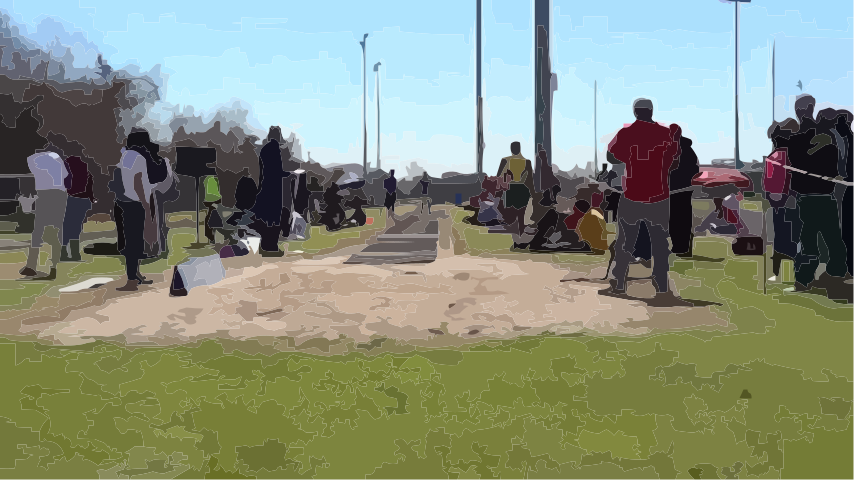
\includegraphics[width=2in, height=1.5in]{images/BCRpdf/frame0.pdf} &
      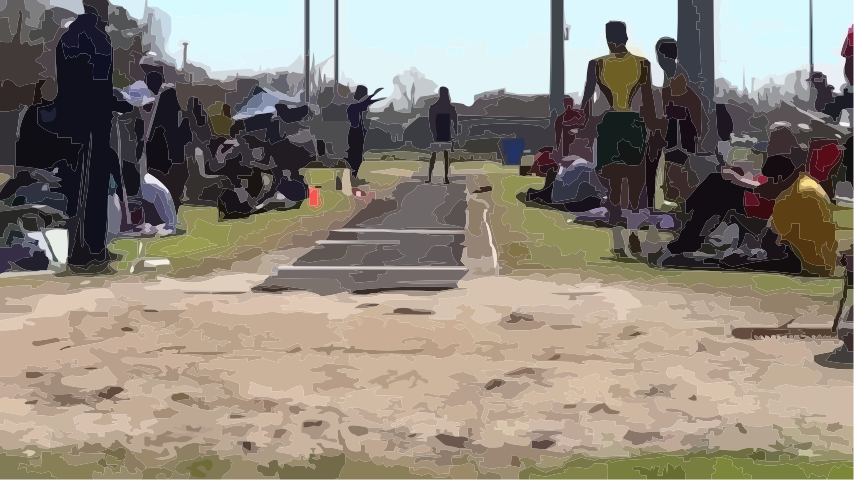
\includegraphics[width=2in, height=1.5in]{images/BCRpdf/frame1.pdf} &
      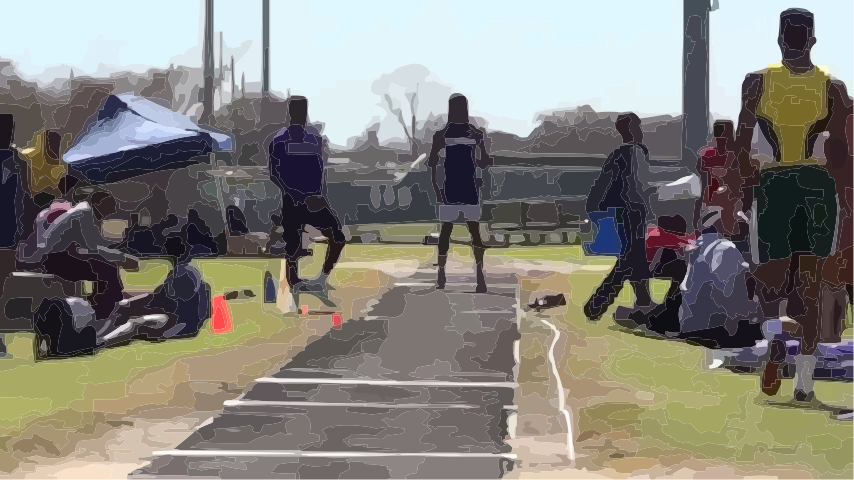
\includegraphics[width=2in, height=1.5in]{images/BCRpdf/frame2.pdf} &
      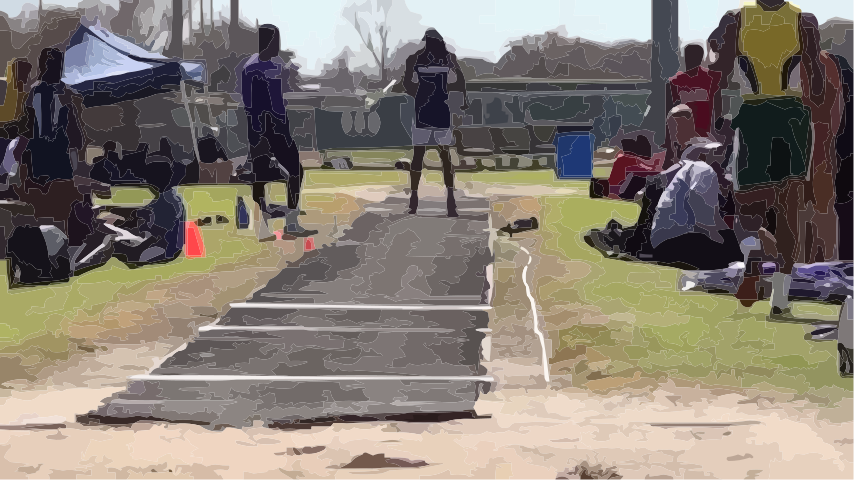
\includegraphics[width=2in, height=1.5in]{images/BCRpdf/frame3.pdf}  &
      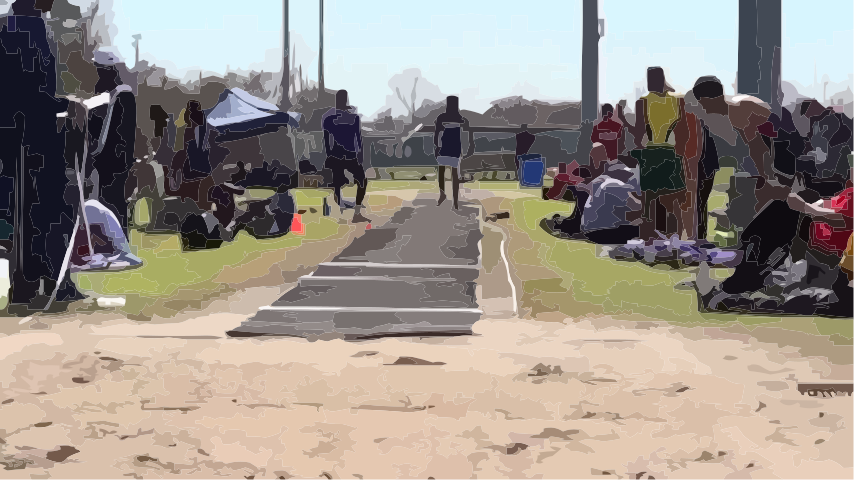
\includegraphics[width=2in, height=1.5in]{images/BCRpdf/frame4.pdf}  &
      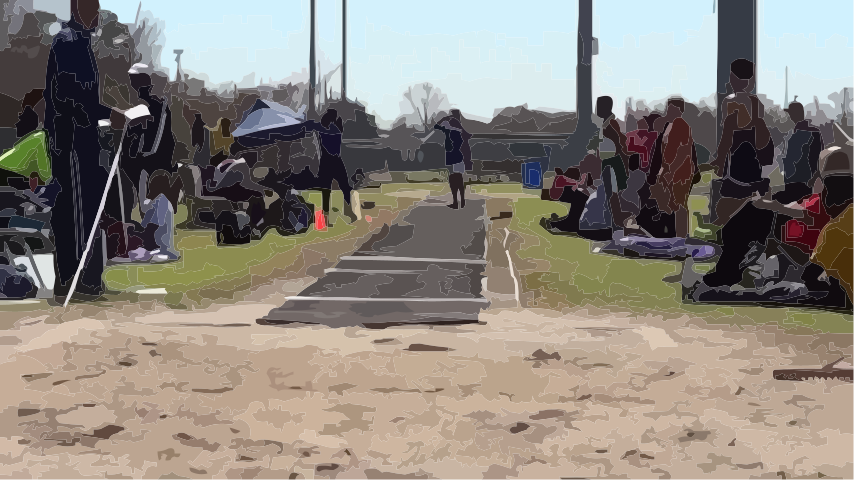
\includegraphics[width=2in, height=1.5in]{images/BCRpdf/frame5.pdf}  &
      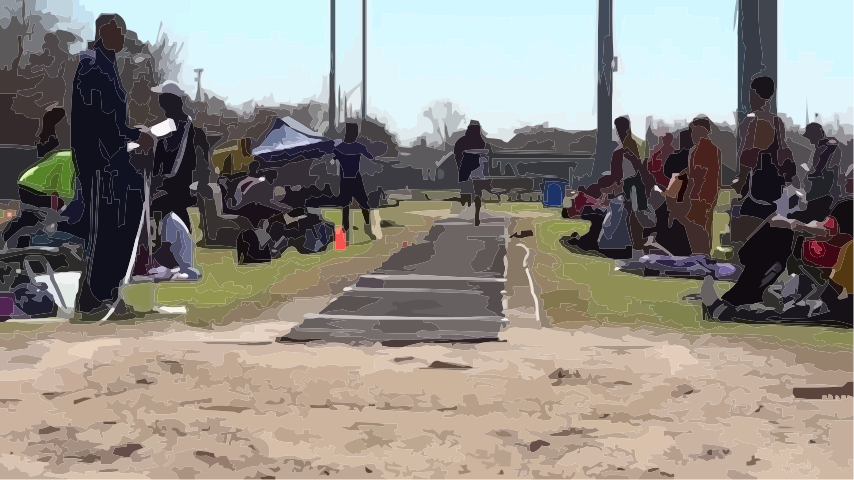
\includegraphics[width=2in, height=1.5in]{images/BCRpdf/frame6.pdf} &
      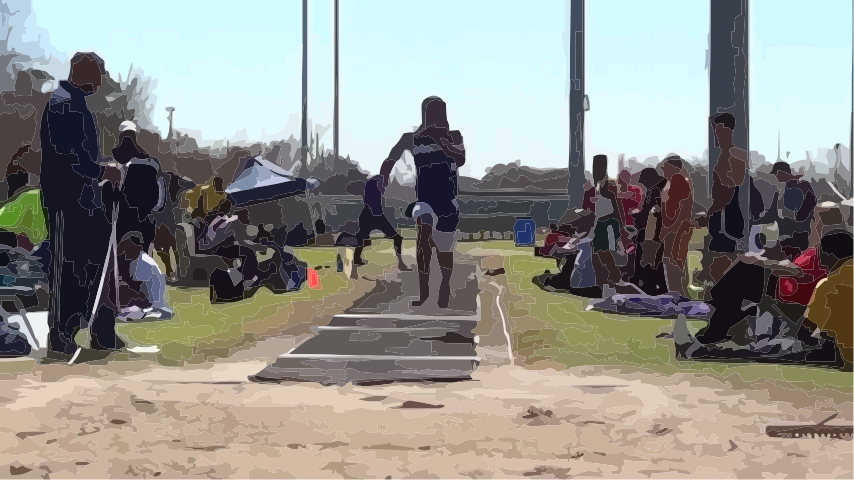
\includegraphics[width=2in, height=1.5in]{images/BCRpdf/frame7.pdf}  &
      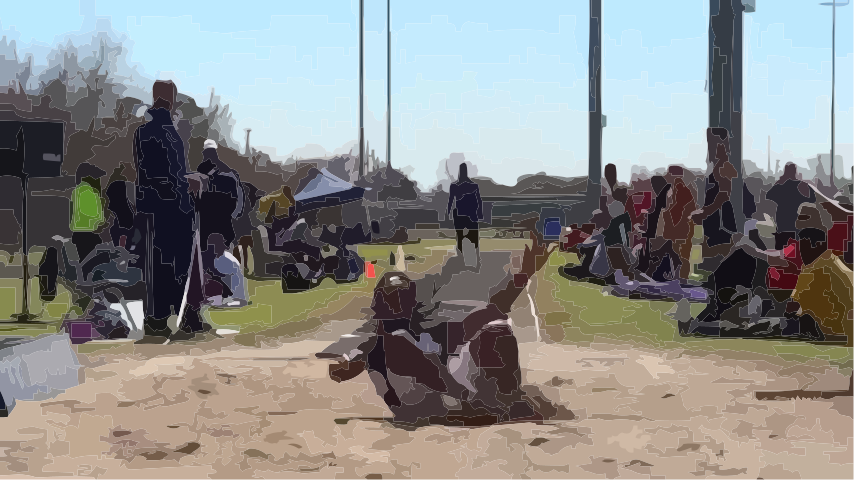
\includegraphics[width=2in, height=1.5in]{images/BCRpdf/frame8.pdf} &
      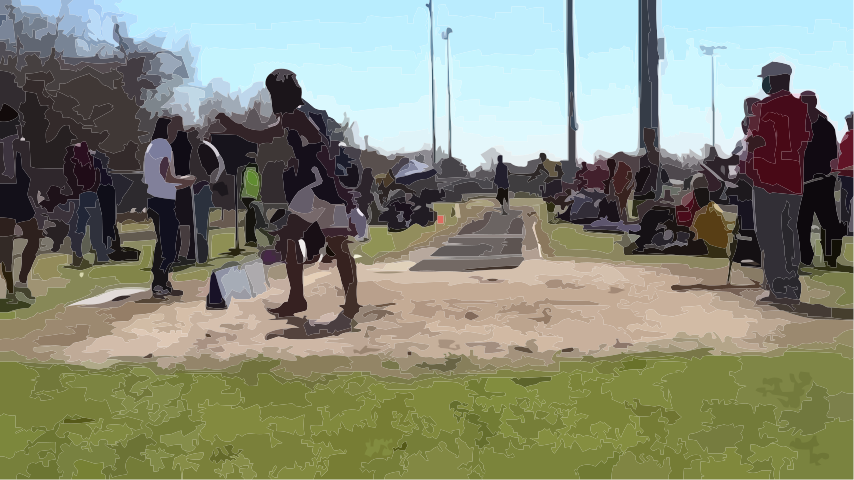
\includegraphics[width=2in, height=1.5in]{images/BCRpdf/frame9.pdf}  \\
    \end{tabular}%
  }
    \captionof{figure}{Video ID v\_BCRFFkvfB\_Q : Shows the video of a man performing a long jump}
    \label{longjump}
\end{table*}

\subsection{Results}
This section interprets and discusses the main findings of our evaluation results. Figures \ref{sofapainting} and \ref{longjump} showcase selected frames from two videos in our test set. Tables \ref{tab:table1} and \ref{tab:table2} and contain their corresponding ChatGPT-generated descriptions obtained using the outputs from each of our tested models. By observing these summaries for accuracy, conciseness, and coherence with the ground truth, we can infer that SwinBERT is likely the best-performing model, followed closely by DenseCap and MART, while our baseline and PDVC models appear to produce inferior quality results.

A closer examination of the evaluation scores listed in Table \ref{tab:table3}, where higher scores indicate better performance, confirms our initial beliefs about the models in general but also reveals new insights about them and the evaluation criteria of the metrics themselves. These values represent the metric score for each model averaged over the scores from all 26 video captions. Higher scores attained by SwinBERT and DenseCap in terms of Cross-Encoders and ROUGE suggest they are better at capturing relationships between the original captions and producing coherent summaries compared to the other models. METEOR scores point towards DenseCap being the most effective at generating summaries that are not only close to the ground truth but also containing a high degree of semantic similarity. As per our expectations, PDVC and the baseline were generally among the worst performing models. Interestingly, the SARI scores did not follow the same trend as the other metrics and revealed some unexpected results. The SARI scores indicate that PDVC performed surprisingly well, while DenseCap and SwinBERT, which performed well on the other metrics and produced more comprehensible summaries, had low scores. This behaviour is visible in Figure \ref{sari-scores}, where PDVC portrays almost contrasting normalized SARI scores for most of the videos against DenseCap, SwinBERT and MART. It is worth noting that SARI evaluates the structural and lexical similarity between the ground-truth and the generated summaries. It is possible that PDVC's summaries had a higher resemblance to the ground-truth values in terms of structure and lexicon, despite being less semantically accurate. Alternatively, it is plausible that SARI may not be equally sensitive to all types of errors or differences between the generated and reference summaries, which could affect the relative rankings of the models. The observed inconsistency may indicate a possible inverse association between SARI scores and model performance. It underscores the significance of using several evaluation metrics to gain a more complete perspective on the models' overall performance. Different metrics measure different aspects of text quality, for instance, ROUGE measures the overlap between generated and reference summaries, while SARI measures the structural similarity between the two. However, the fact that the scores for all the models evaluated are low and ranged closely indicates that no model performed exceptionally well compared to the rest and that there is still room for improvement. It also suggests that the current state-of-the-art models may not be significantly better than simpler baseline models in terms of their ability to generate high-quality summaries. It is possible that these scores were biased by the limited diversity as represented in the 26 videos we evaluated the models upon, or that models such as SwinBERT and DenseCap were unable to adapt to the requirements of the video features, despite being trained on similar datasets.

\begin{figure}[htbp]
\centering
\centerline{\includegraphics[scale=0.38]{images/sari scores.png}}
\captionsetup{justification=centering}
\caption{Visual representation of the SARI scores of each model on the 26 test videos}
\label{sari-scores}
\end{figure}

\begin{table*}[!htbp]
    \centering
    \renewcommand{\arraystretch}{1.5}
        \begin{tabular}{|p{2cm}p{14cm}|} 
             \hline
             \textbf{Ground Truth} & \textit{Man is in a living room painting a couch with purple spray.
man paint the cushions of the couch on top of paperboard.}\\
             \hline
             \textbf{Baseline}  & A person is seen sitting on a tan chair with a man standing behind them. A young girl is shown climbing a rock wall, and a man is climbing up an icy wall while attached to safety ropes. Another person is sitting inside a room. There's a painting on the wall where a child with a green shirt is sitting. A little boy in blue shorts is seen climbing a bathtub covered in bubbles. Lastly, a man is shown looking down through a window. \\
             \textbf{DesnseCap } & In the video, a woman can be seen kneeling down next to a table and putting a box on the floor. She carefully places a piece of paper into the box and then sets it on the table. She begins to place various objects around the table and in the box, taking care with each item. At one point, she speaks to the camera while kneeling on the floor. After finishing with the objects, she begins to wrap the box in another box, ensuring that it is secure. She then places the wrapped box on the table and starts to clean the floor with a rag. Later, she continues to wrap other boxes while kneeling on the floor and places them on the table. A man is also briefly seen holding a rag and a mop, presumably helping with the cleaning.\\
             \textbf{MART}  &  The video opens with a woman standing in front of the camera, holding a box. She speaks to the camera, explaining something about the box, before placing it on a nearby table. Next, the woman grabs a sheet of paper and puts it on the floor. She takes out some paint and begins to create a colorful pattern on the paper, using a brush. As she paints, she continues to speak to the camera, perhaps discussing her painting process or sharing some thoughts on creativity. The camera captures her movements and the details of her painting as she works. Eventually, she finishes her artwork and holds it up to the camera, showing off her creation. The video ends with the woman thanking the viewer for watching and perhaps inviting them to try their own painting project.\\
             \textbf{PDVC}  & The video starts with a woman speaking to the camera. Then, there is a black screen with white words appearing. After that, the credits of the video are shown several times, followed by a white screen with a white screen appearing, and then a black screen with a white screen appearing again.\\
              \textbf{SwinBERT}  & A man is demonstrating how to use a spray bottle to paint a couch. He holds the spray bottle and applies the paint evenly on the couch, covering every inch of the surface. He shows how to use a smooth, sweeping motion to avoid any uneven patches or drips. The couch gradually transforms from its previous color to a new, vibrant shade. The man takes care to ensure that the paint is applied evenly and covers the entire couch. He completes the process and steps back to admire his work, pleased with the results.\\ 
             \hline
        \end{tabular}
          \caption{Video ID v\_IlN\_XipVf44. Compares the ground truth value for \textit{'Man paintaining a couch'} from ActivityNet with the descriptions obtained from each of our models, after running them through ChatGPT}
    \label{tab:table1}
\end{table*}
\begin{table*}[!htbp]
    \centering
    \renewcommand{\arraystretch}{1.4}
        \begin{tabular}{|p{2cm}p{14cm}|} 
             \hline
             \textbf{Ground Truth} & \textit{A large group of people are seen standing around an area with a man standing in front. The man then begins running down the track with others watching. Finally he jumps into a pit in the end and others measure his throw.}\\
             \hline
              \textbf{Baseline} & A group of people sit on the edge of a march near a grassy body of water, while two others sit in line at the edge of a road, and four men with motorcycles are on a field in a park, while a man skateboards on the ground and people watch, and another man walks on the beach near some rocks, and two people sit in chairs at the park, and a man grinds down a handrail, and skateboard racers jump over a bridge, and two men are on some sand, and two people in brown jackets are running along a rural road. \\
              \textbf{DesnseCap } & A man is standing before a track, ready to take off. His eyes are focused ahead as he takes a deep breath, preparing himself mentally for what's to come. Suddenly, he begins to run down the track, his powerful legs propelling him forward with each step. He moves with a determined stride, his form sleek and athletic as he races towards his goal. Around him, a large group of people watches, their cheers and applause pushing him to go faster and harder. As he reaches the end of the track, he triumphantly raises his arms in the air, a look of satisfaction on his face. He then walks away from the camera, his head held high, knowing he has achieved something great. \\
              \textbf{MART } &  A man is standing on a track and begins walking away. He continues walking and eventually jumps off the ground before walking away from the camera.\\
              \textbf{PDVC}  & Based on the given text, it appears that the video ends with the words on the screen. Throughout the video, there are multiple instances where a woman is seen speaking to the camera, and the credits of the video are shown several times.\\
              \textbf{SwinBERT}  & A man performs a long jump and lands in a sand pit as a few spectators watch him in action.\\ 
             \hline
        \end{tabular}
    \caption{Video ID \- v\_BCRFFkvfB\_Q. Compares the ground truth value for \textit{'Man performing a long jump'} from ActivityNet with the descriptions obtained from each of our models, after running them through ChatGPT}
    \label{tab:table2}
\end{table*}
\begin{table*}[!h]
    \centering
    \renewcommand{\arraystretch}{1.2}
        \begin{tabular}{|p{2.8cm}p{2.3cm}p{2.3cm}p{2.3cm}p{2.3cm}p{2.3cm}|} 
             \hline
             \textbf{Evaluation Metric} & \textbf{Baseline} & \textbf{DesnseCap} & \textbf{MART} & \textbf{PDVC} & \textbf{SwinBERT} \\ 
             \hline\hline
             \textbf{Cross-Encoders} & 0.1537 &  0.2646 & 0.2396 & 0.1329 & 0.3085 \\ 
             \textbf{ROUGE} & 0.1896 & 0.2407 & 0.2439 & 0.1971 & 0.2459\\
             \textbf{METEOR} & 0.1949 & 0.2614 & 0.2510 & 0.1619 & 0.2483\\
             \textbf{SARI} & 63.038 & 48.282 & 64.980 & 74.478 & 61.914 \\
             \hline     
        \end{tabular}
    \caption{Comparison of evaluation metrics for different models}
    \label{tab:table3}
\end{table*}

